\section{CHAPTER 9: FLOW METERS}

\subsection{Overview:}
Flow meters are very important measuring instruments in steam systems, allowing real-time flow of steam in industrial pipelines. These instruments have become very crucial in the monitoring of steam consumption patterns, enhancing energy use, and ensuring that equipment operates at optimal performance. The technology has quite a few variants based on differing operating principles: differential pressure mechanisms, vortex formation, ultrasonic wave propagation, and thermal mass measuring techniques. With accurate flow rate determination, the instruments allow the operators of such facilities to make complete system assessments, identify potential inefficiencies, and data-driven optimization of steam management.

\subsection{Electromagnetic Flow meter:}
An electromagnetic flow meter is a modern answer to the measurement of conductive fluid flow in industrial applications. This technology applies Faraday's principle of electromagnetic induction to a well-thought-out design. Its construction has coils placed at specific points creating magnetic fields through the non-conductive pipe sections.

\begin{figure}[h!]
    \centering
    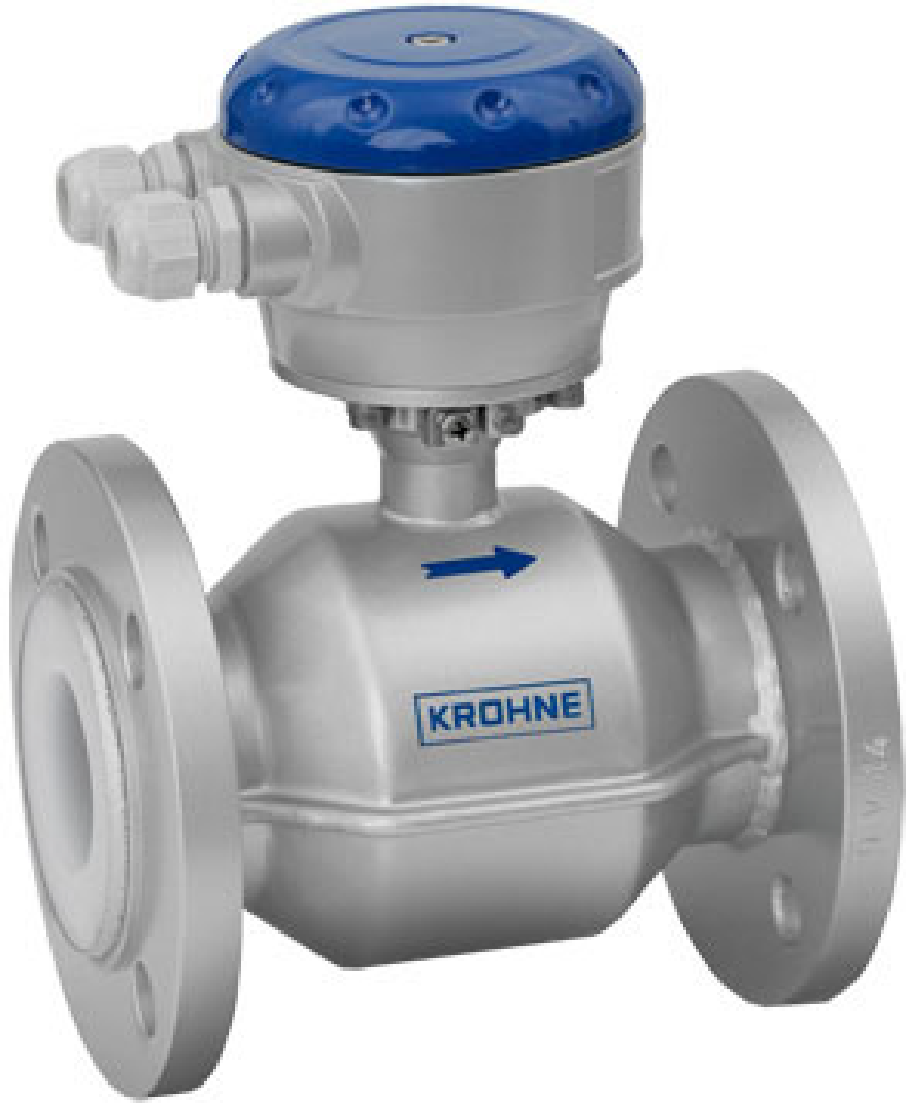
\includegraphics[width=1.8in,height=2.31944in]{figs/flowmeters/image1.png}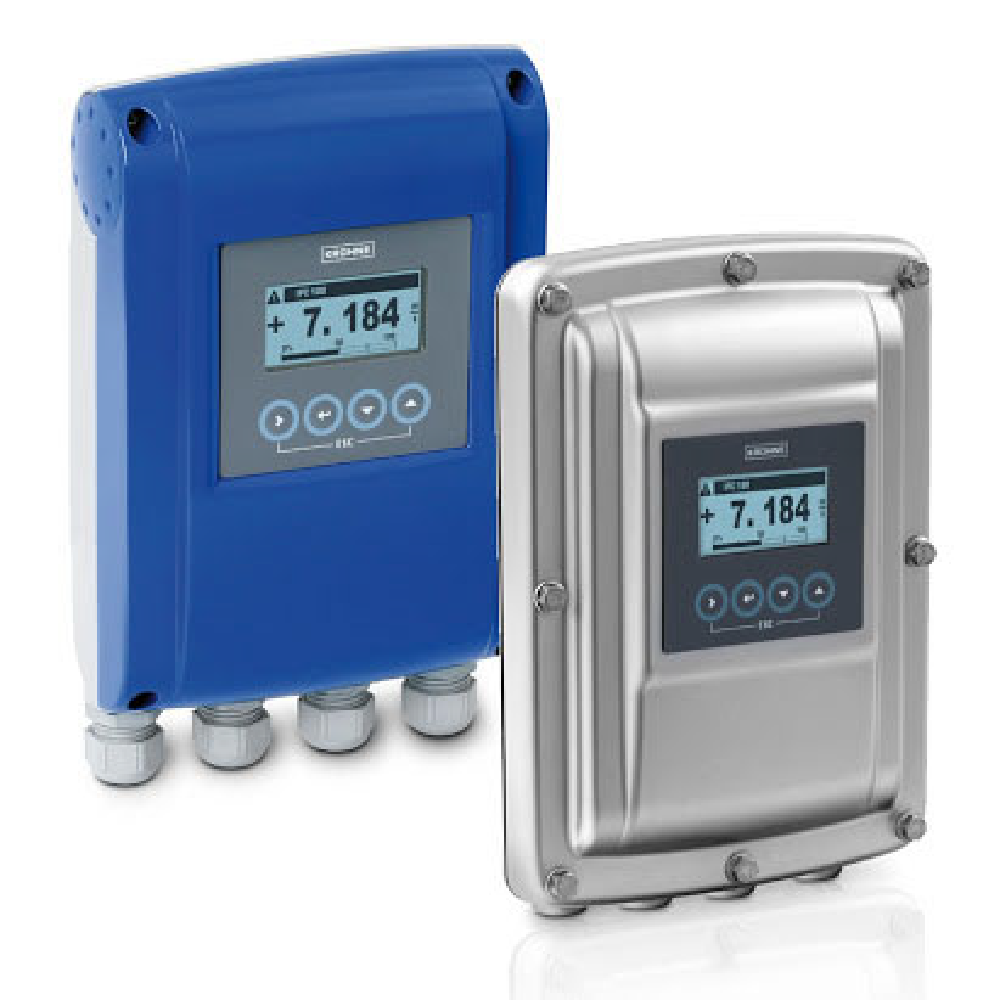
\includegraphics[width=2.0in,height=2.31944in]{figs/flowmeters/image2.png}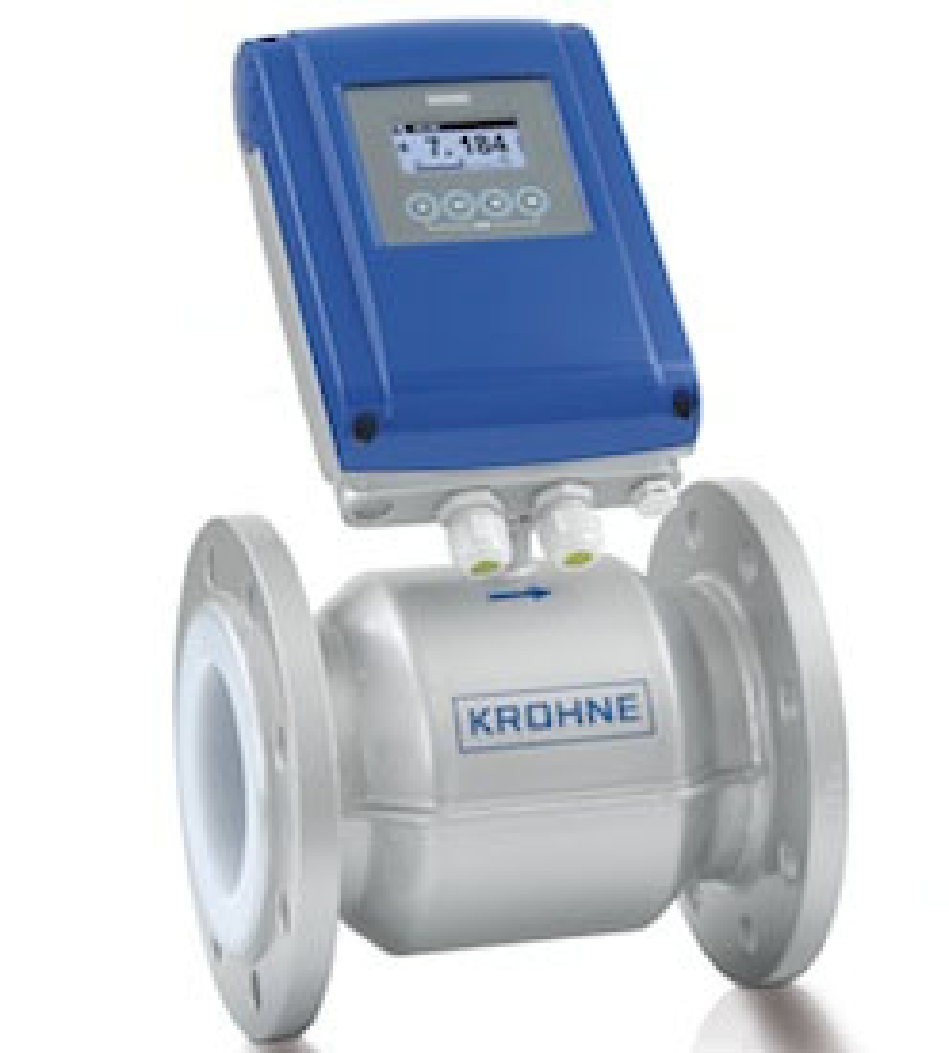
\includegraphics[width=2.0in,height=2.31944in]{figs/flowmeters/image3.png}
    \caption{Electromagnetic Flow Meters (a) Compact version; (b) Remote display.}
    \label{fig:ElectricFlowMETERS}
\end{figure}

When conductive fluids flow through these magnetic fields, an electromotive force is produced which is directly proportional to the fluid velocity. These designs provide critical advantages for industrial applications: namely, excellent accuracy at all operating conditions and low maintenance as there are no moving parts. Robust construction provides reliable performance in difficult industrial environments, while the lack of mechanical parts contributes to longer operating life and reduced periods of maintenance.

\subsection{Vortex Flow meter:}

The vortex flow meter is the new solution for fluid movement measurement allowing the measurement of fluid flow movement in different industries. It is based on the von Karman effect, in which a fluid flow over a geometric obstruction located at a suitable location in the flow generates alternating vortices. These disturbances are predictably induced and these causally link the frequency of the vortices to the velocity of the flow.

The technology is based on advanced piezoelectric sensing elements that detect and interpret the generated vortex forms. The meter design is also very adaptable concerning the various types of media employed such as liquid, gas, or steam. New possibilities in industrial processes with this device are more precise measurements with large operation ranges and negligible effects on the pressure properties of the system.

\begin{figure}[h!]
    \centering
    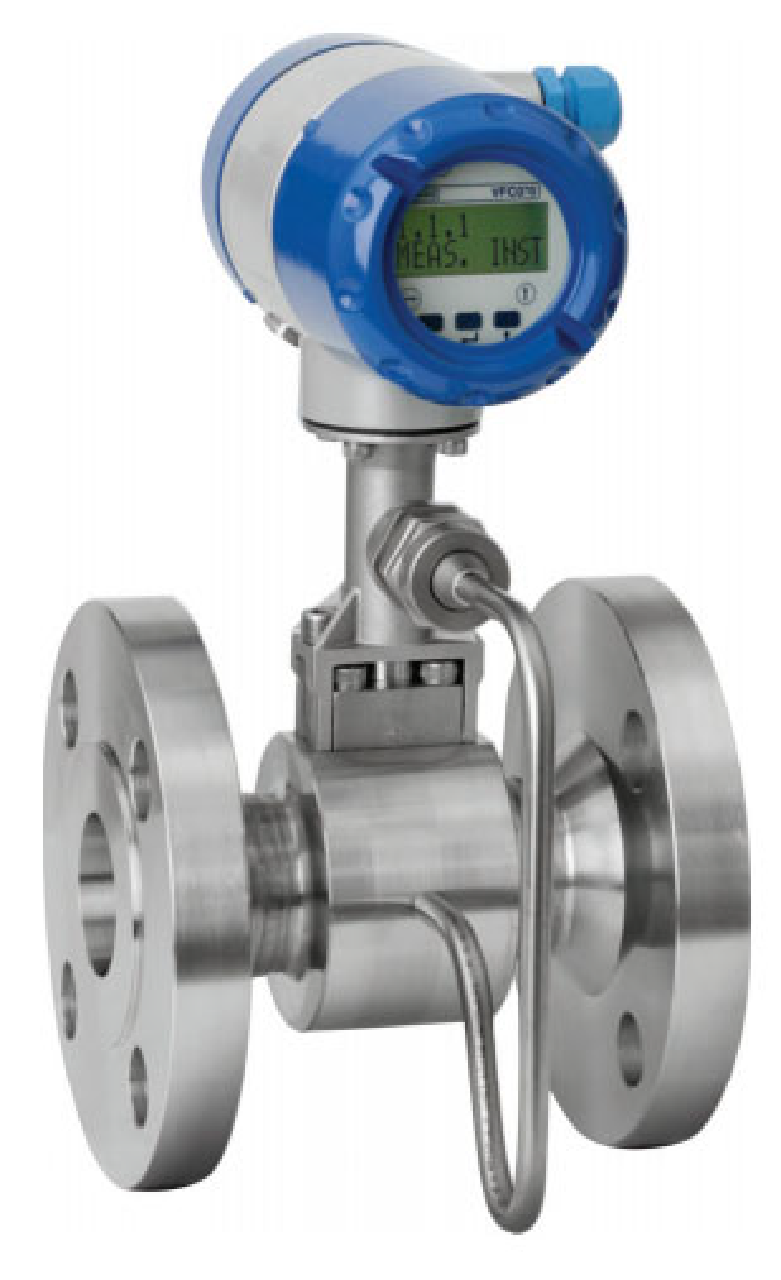
\includegraphics[width=1.41806in,height=2.31944in]{figs/flowmeters/image7.png}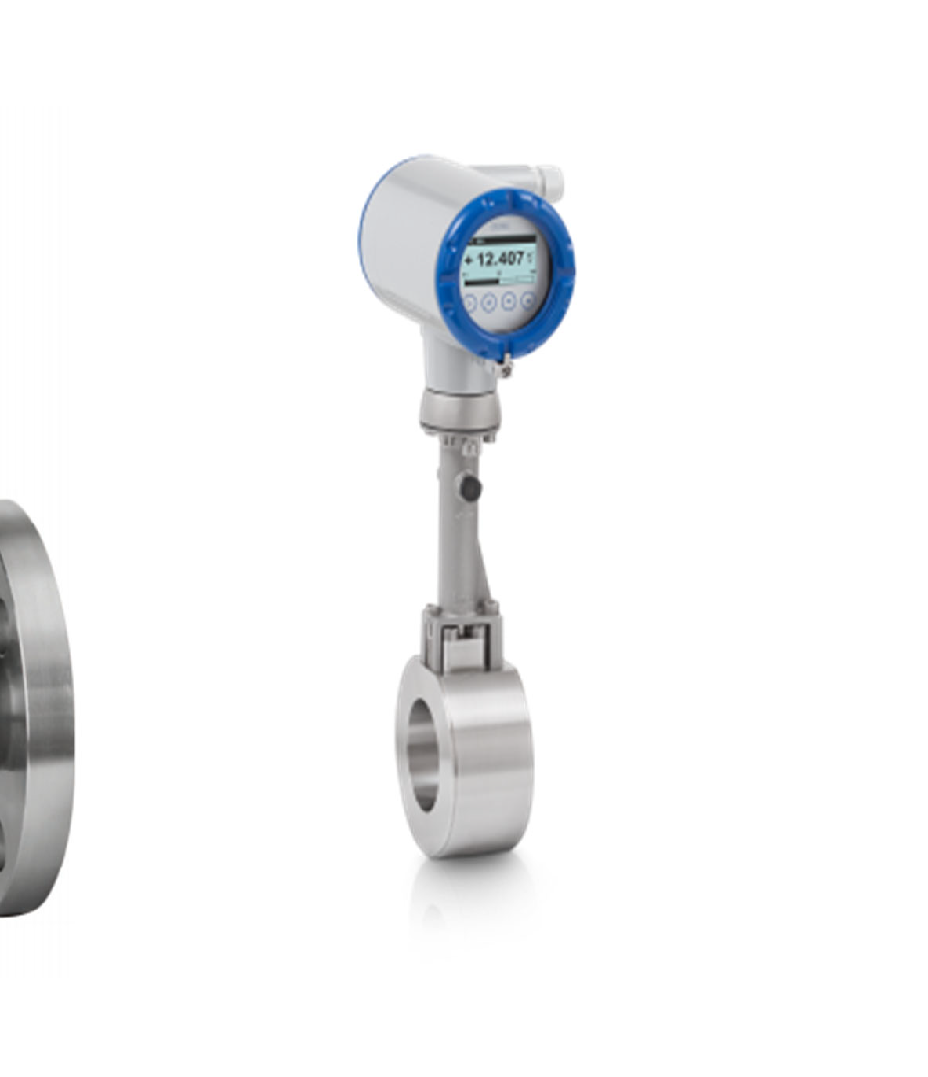
\includegraphics[width=1.99792in,height=2.31944in]{figs/flowmeters/image8.png}
    \caption{Various types of Vortex Flow Meters}
    \label{fig:electric_flowmeters}
\end{figure}

\subsection{Coriolis Mass Flow meter:}

Coriolis mass flow meters utilize fundamental physical principles to achieve precise measurement of mass flow and are the cutting-edge technology of the measuring device industry. The devices are made of vibrating flow tubes that touch the stream of fluids that pass through it. The interaction between the flow within such tubes and the rotation of the Earth results in the Coriolis force that twists the oscillating tubes whenever the fluid passes through them.

This specialized construction therefore means that mass flow rates can be correlated directly with the small tube flexes detected by sensor arrays. This design approach yields remarkable benefits: unmatched measurement accuracy, extensive operating ranges, and the ability to measure mass flow without regard for changes in fluid density, viscosity, or temperature.


\begin{figure}[h!]
    \centering
    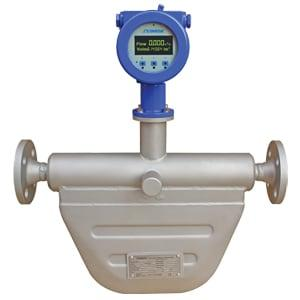
\includegraphics[width=2.31944in,height=2.31944in]{figs/flowmeters/image11.jpg}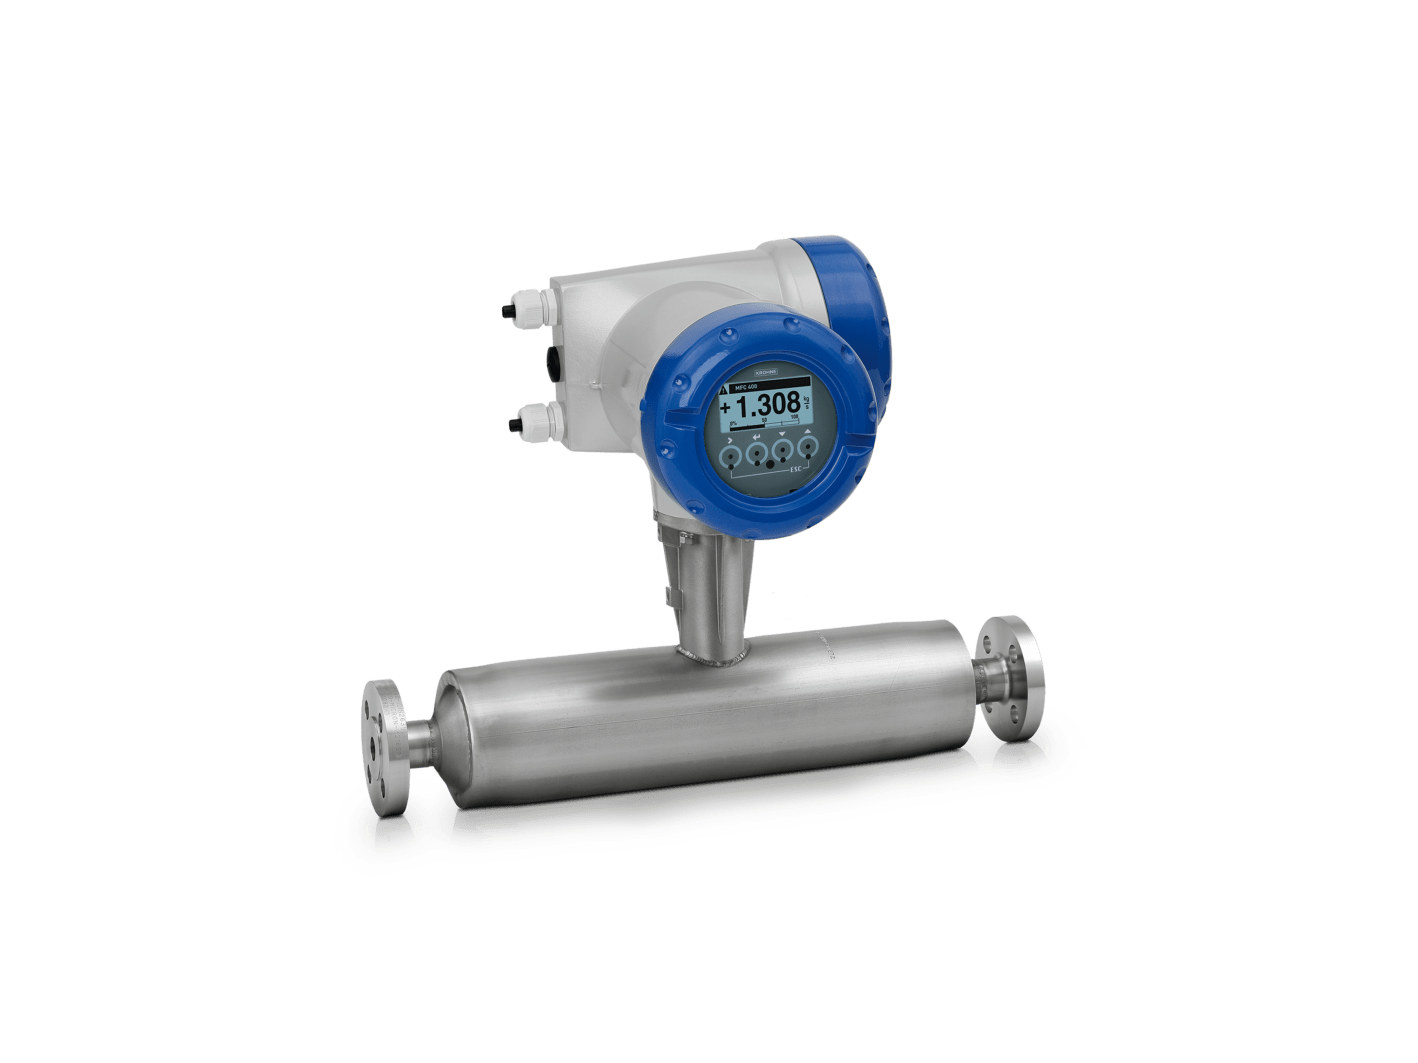
\includegraphics[width=3.09375in,height=2.31944in]{figs/flowmeters/image12.png}
    \caption{Various types of Coriolis Mass Flow meter.}
    \label{fig:Various types of Coriolis Mass Flow meter.}
\end{figure}

\subsection{Variable Area Flow meter:}
Variable area flow meters, also called rotameters, are simply practical meters for measuring flows in industrial applications. The working principle of these meters is incredibly simple; a float that is very carefully calibrated rides inside a precision-tapered tube, where it can move up and down depending on the conditions of flow. When flow is increased, the float will rise; when flow decreases, it will fall, thus constantly changing according to the changes in flow conditions.

\begin{figure}[h!]
    \centering
    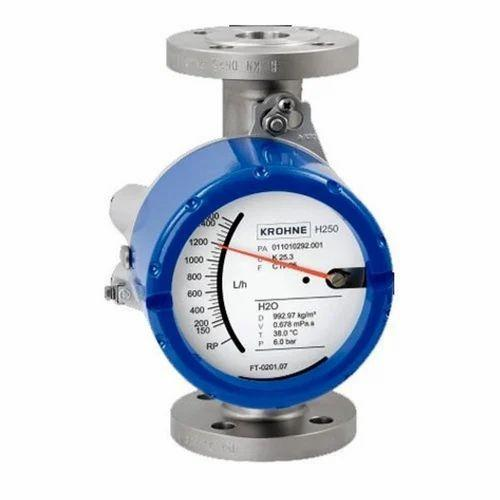
\includegraphics[width=0.45\linewidth]{figs/flowmeters/image15.jpg}
    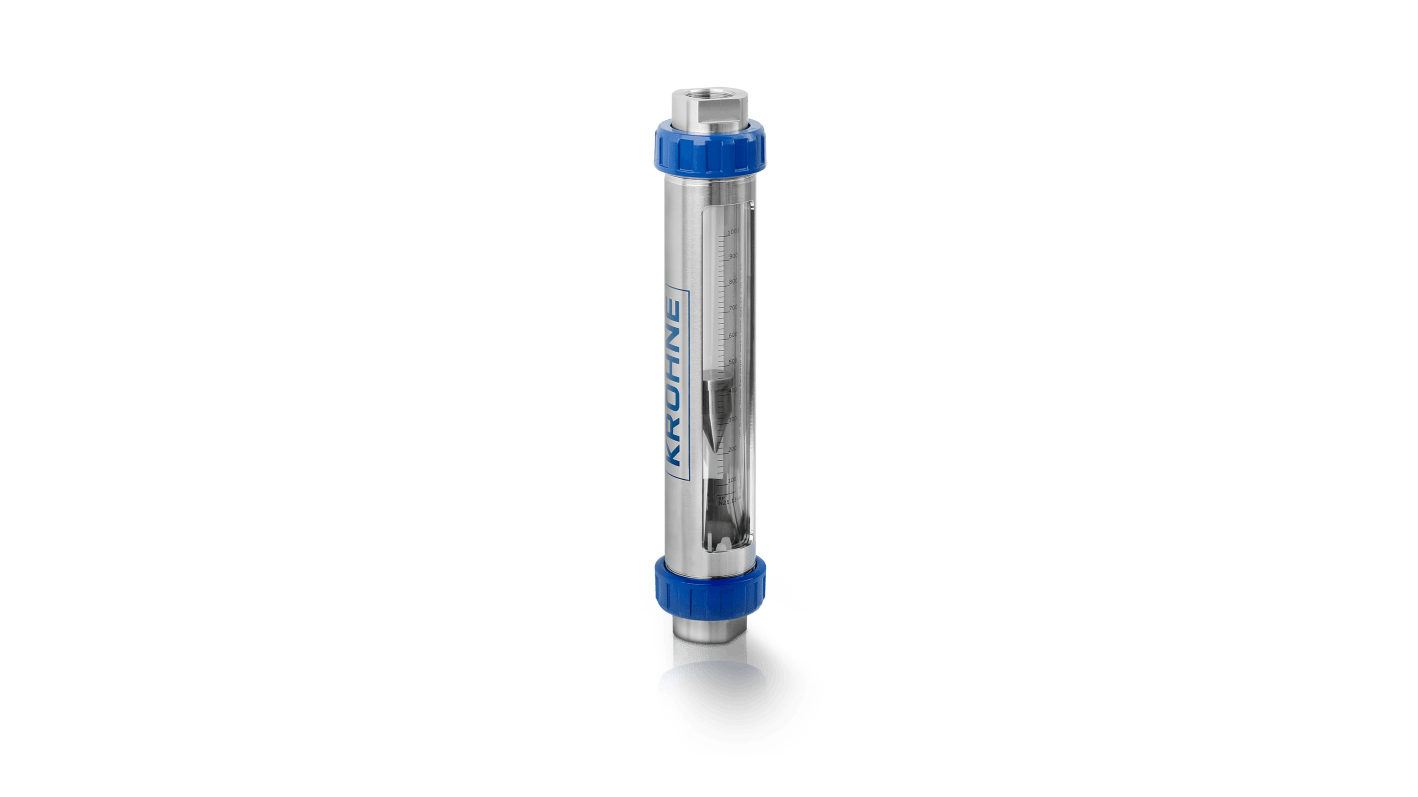
\includegraphics[width=0.8\linewidth]{figs/flowmeters/image16.png}
    \caption{Variable Area Flow Meters (Rota Meter)}
    \label{fig:rota_meter}
\end{figure}

This has some obvious advantages in a purely mechanical way: cheapness, minimal installation needs, plus visual feedback. These devices are found in all low or high-pressure applications, but they are highly sensitive in performance characteristics to changes in the fluid properties: density, viscosity, and temperature variations.

\subsection{Orifice Type Flow meter:}
An orifice meter flow measurement is a very easy way of measuring the flow of liquids or gases through pipes. It has a very simple yet ingenious idea—consider a plate that has a hole in it and is placed inside a pipe. When the fluid flows through this hole, it causes a pressure difference or head between the front and back of the plate. This difference is measured by special pressure sensors placed on both ends of the plate. The flow rate of the fluid can then be estimated by using some mathematics based on Bernoulli's principle. While this type of meter has the advantages of being very simple and easy to install, there is an intrinsic disadvantage associated with it—it tends to give a small pressure drop, and flow may have to be recalibrated to make it accurate.


\begin{figure}[h!]
    \centering
    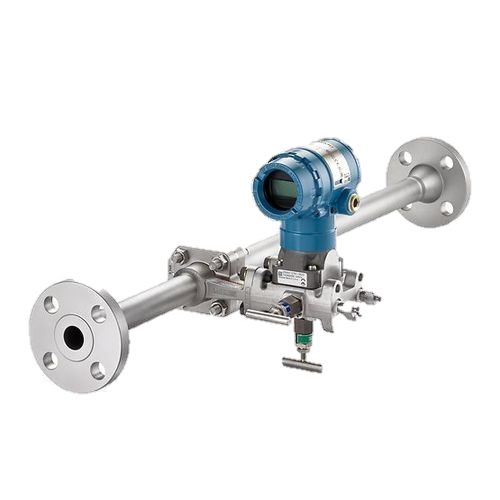
\includegraphics[width=0.8\linewidth]{figs/flowmeters/image19.png}
    \caption{Orifice type flow meter.}
    \label{fig:orifice_flow_meter}
\end{figure}


\subsection{Positive Displacement Flow meter:}
This flow meter works much like filling and emptying cups of known size. The process of measuring fluid flow comprises trapping fixed amounts of liquid in special chambers and letting it out. It counts the number of times these chambers fill and empty, and the meter can calculate how much fluid passes through. Just like counting cups of water, but done automatically and continuously. 

\begin{figure}[h!]
    \centering
    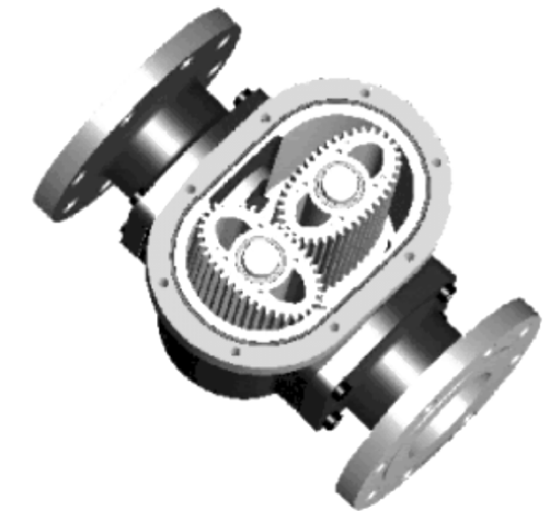
\includegraphics[width=2.50105in,height=2.32in]{figs/flowmeters/image20.png}
    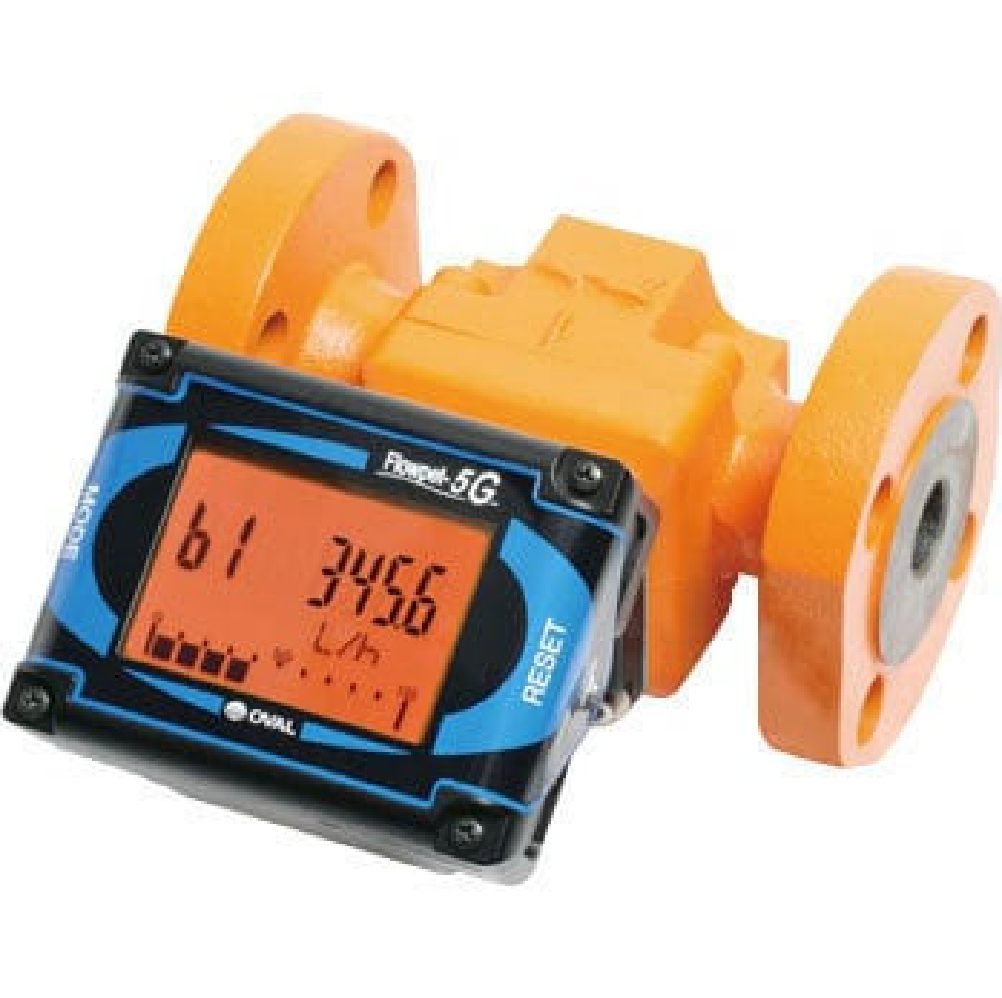
\includegraphics[width=2.33107in,height=2.32in]{figs/flowmeters/image21.png}
    \caption{Positive Displacement Flow meter}
    \label{fig:Positive Displacement Flow meter}
\end{figure}


\subsection{Open channel Flow meter:}
These flow meters are special because they register the velocity of water along its free surface from open passages like rivers, streams, and canals. The converse of other flow meters that operate in closed pipes is that these meters must operate in an open environment of water with a free surface to the atmosphere. They can use several clever ways to tell the flow, including measuring velocity, sonic flow, and pressure changes in water.


\begin{figure}[h!]
    \centering
    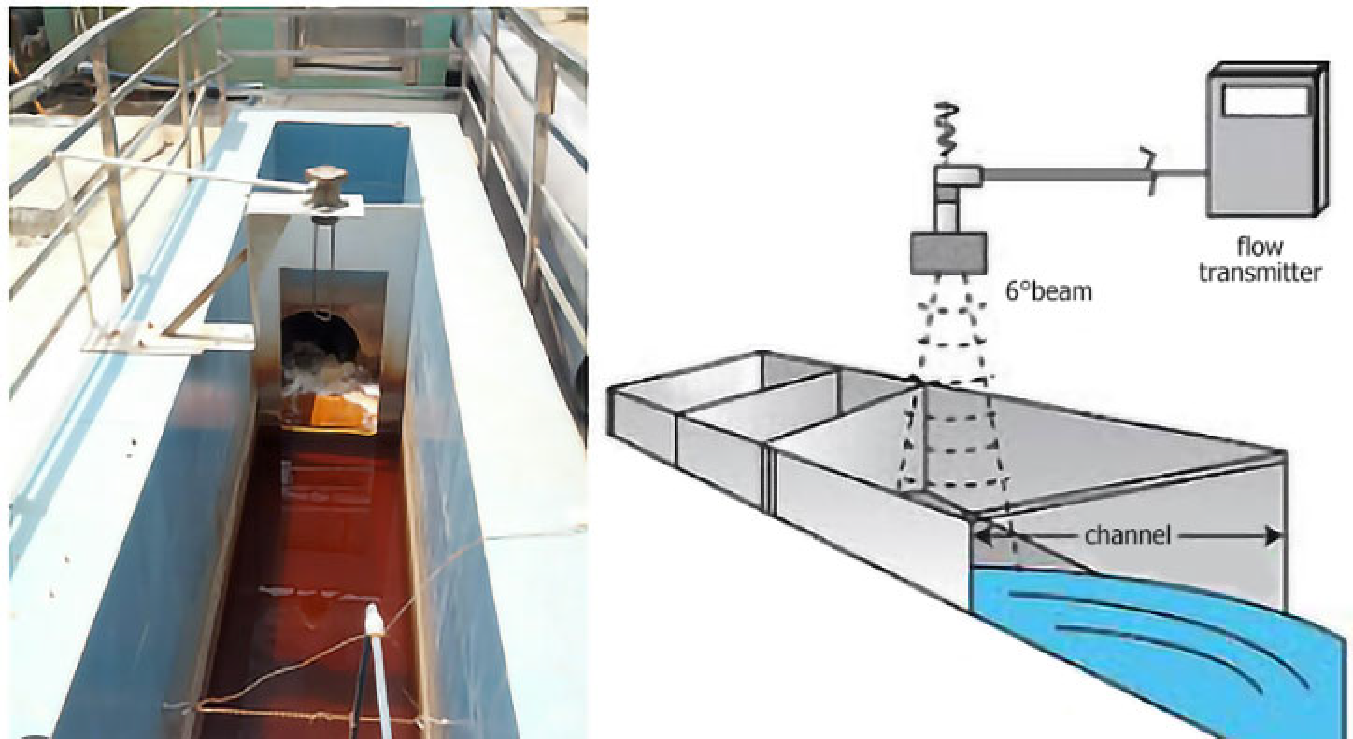
\includegraphics[width=0.8\linewidth]{figs/flowmeters/image22.png}
    \caption{Open channel flow meters}
    \label{fig:Open channel flow meters}
\end{figure}




\subsection{Turbine type Flow meter:}
This turbine flow meter carries out its operating principle very similar to what happens when a small water wheel is placed into a stream. It has a small wheel with blades directed toward the passing flowing fluids. On moving, it causes blades (wheels) to revolve. The not-so-good point is the velocity of fluid flow increases, and that will increase the speed of spinning blades. Thus, knowing how fast the blades rotate can determine at what speed fluid is flowing through the pipe. The main advantage of such a meter is better accuracy in measurement in various industries.

\begin{figure}[h!]
    \centering
    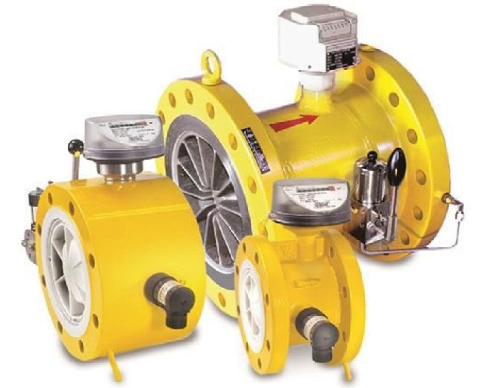
\includegraphics[width=2.18787in,height=1.76042in]{figs/flowmeters/image23.png}
    \caption{Turbine type flow meter.}
    \label{fig:Turbine type flow meter}
\end{figure}

